\chapter{Evaluation}
\label{ch:Evaluation}

\section{Analysis: First approach}
\subsection{Experiments setup}
\label{exp}

To evaluate the model, we run tests on a subset of the AIDA dataset presented by \cite{hoffart-etal-2011-robust}. This dataset is based on CoNLL 2003\footnote{https://www.conll.org} and it contains 1393 documents of Reuters news in these documents there are ~27.000 mention-entity pairs to be found.

The documents included in this dataset are divided into three sets; A training set containing ~18.500 pairs from which 4085 are unique entities, and two others containing respectively 4785 and 4458 pairs, namely evaluation/validation sets. The number of documents in each set is 946, 216, and 230 respectively.\newline

The knowledge base from which we extracted the embeddings, was constructed from the March 2021 version of the DBpedia. Using the Pytorch-BigGraph library\footnote{https://github.com/facebookresearch/PyTorch-BigGraph}, for each entity a 100-dimensional embedding vector was computed\footnote{Embeddings were computed using https://github.com/nikit91/configs/blob/master/kge/pbg/dbp21-03\_config\_cpu\_transe\_dot.py}.\footnote{https://hobbitdata.informatik.uni-leipzig.de/KGE/PBG/DBpedia-2021-03/readme.txt}. From this Knowledge base we took 1.32M entities, with these we build our index to be queried. \newline

We used the Adam optimization algorithm\cite{ADAM} to optimize the weights of the model. And to mitigate the problem of exploding gradient\footnote{https://deepai.org/machine-learning-glossary-and-terms/exploding-gradient-problem} we use the gradient clipping with norm method with a configurable maximum value.\newline

As a performance metric, we computed the recall percentage when retrieving the closest 50 candidates from the index given the output of the model as a query vector.\newline
We used the following formula:
\begin{equation}
Recall@50 = \dfrac{|Mentions for which golden entity is present in the candidates set|}{|All the mentions for which entities should be retrieved|}
\end{equation}
from the set of mentions present in the input documents we did not count the ones for which no embeddings were present in the index.\newline

\subsection{Analysis of training and testing}
As discussed in the previous chapter for the training methods we opted for the negative sampling approach and the direct optimization of the sum of cosine and euclidean distance. After pre-processing and index compilation, we initialized the following variables:
\begin{itemize}
\item{\textit{Model's parameters}: input-size=768; output-size=100; layers=12, attention-heads=12; forward-expansion=4; dropout=0.1}
\item{\textit{Training parameters}: epochs=3; learning-rate=$1\cdot e^{-6}$; batch-size=8}

\end{itemize}

We evaluated two models on the Dataset AIDA\_TESTA. This dataset contained in total, 4785 pairs out of which 1073 are unique entities. From these, we could extract 3852 for which we had embeddings in our index.\newline
In figure\ref{training1st} we observe the evolution of the average cosine similarity of every 10th batch during training. These models were given the embedding vectors of the wordpieces that only made the mention's surface form and each was trained with a different loss function. We set the batch size for this round of training to 8, and the maximum value for the gradient clipping with normalization to 1.\newline

\begin{figure}[h]
\centering
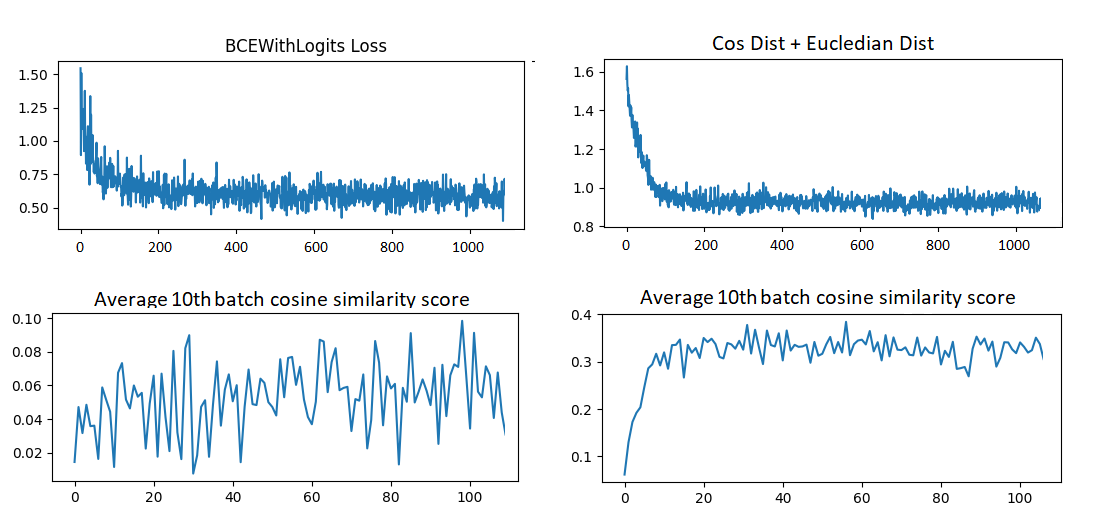
\includegraphics[width=15cm]{figures/NoContextEpoch0.png}
\caption{Average cosine similarity evolution over the training.}
\label{training1st}
\end{figure}

As we can see the model gets better the more examples it processes, however, as shown in table \ref{1stRound} the recall@50 (recall at recovered sets of 50 candidates) is very insignificant.\newline


\begin{table}[h]
\centering
\begin{tabular}{ |p{3cm}||p{2.5cm}||p{2.5cm}|p{2.5cm}|p{2.5cm}|}
 \hline  
  Recall@50 on AIDA\_A & Recalled entities & Recall & Average cos sim & Maximum cos sim\\
 \hline 
 Cos + Euc dist & 126 & 0.03 & 0.16 & 0.58  \\
 \hline
 BCE with Logits & 11 & 0.002 & 0.16 & 0.43\\
 \hline
\end{tabular}
\caption{Results of the first round of training }
\label{1stRound}
\end{table}

In sight of these results, we decided not to test any further models without considering the context of the mentions, and to train the model solely relying on the distance-based loss function. We added the embeddings of the tokens surrounding the mention and with the same parameters as before, we trained and tested the models with the new input vectors.\newline

\begin{figure}[h]
\centering
\includegraphics[width=15cm]{figures/COSSME\_Context.png}
\caption{Average cosine similarity evolution over the training (including mentions' context).}
\label{training2}
\end{figure}

During training, we made similar observations to the first case. i.e. a declining loss curve and an ascending cosine similarity score Figure \ref{training2}. Although there was a slight improvement in the model's performance compared to when the input lacked information about the context, 
the recall percentage was still too low (Table\ref{2ndRoundA}).

\begin{table}[h]
\centering
\begin{tabular}{ |p{3cm}||p{2.5cm}||p{2.5cm}|p{2.5cm}|p{2.5cm}|}
 \hline   
  Recall@50 & Recalled entities & Recall  & Average cos sim & Maximum cos sim\\
 \hline 
 AIDA\_A & 110 & 0.028 & 0.17 & 0.57 \\
 \hline
 AIDA\_B & 107 & 0.027 & 0.15 & 0.54\\
 \hline
\end{tabular}
\caption{Results of training with the CosEuc distance loss}
\label{2ndRoundA}
\end{table}

Up to this point, we trained all models with gradient clipping with normalization and set the max value to 1. We conducted further testing with different values. At one point with a higher max\_norm value (i.e. 10, table\ref{3rdRound}) and at another without clipping the gradients (table \ref{3rdRound1}).\newline


\textbf{Gradient clipping max\_norm=10}
\begin{table}[h!]
\centering
\captionsetup{justification=centering,margin=2cm}
\begin{tabular}{ |p{3cm}||p{2.5cm}||p{2.5cm}|p{2.5cm}|p{2.5cm}|}
 \hline   
  Recall@50 & Recalled entities & Recall  & Average cos sim & Maximum cos sim\\
 \hline 
 AIDA\_A & 179 & 0.06 & 0.19 & 0.6 \\
 \hline
 AIDA\_B & 177 & 0.04 & 0.16 & 0.58\\
 \hline
\end{tabular}
\caption{Results of training with the CosEuc distance loss and gradient clipping max\_norm set to 10}
\label{3rdRound}
\end{table}

\textbf{no Gradient clipping}
\begin{table}[h!]
\centering
\captionsetup{justification=centering,margin=2cm}
\begin{tabular}{ |p{3cm}||p{2.5cm}||p{2.5cm}|p{2.5cm}|p{2.5cm}|}
 \hline   
  Recall@50 & Recalled entities & Recall  & Average cos sim & Maximum cos sim\\
 \hline 
 AIDA\_A & 113 & 0.02 & 0.15 & 0.57 \\
 \hline
 AIDA\_B & 149 & 0.05 & 0.17 & 0.57\\
 \hline
\end{tabular}
\caption{Results of training with the CosEuc distance loss and no gradient clipping}
\label{3rdRound1}
\end{table}

At this stage, we noticed that most of the predicted entities are in the 50-most frequent entities in the training set. For example, the entity "\textit{http://dbpedia.org/resource/London}" was correctly predicted 100\% of the time. \newline
Other entities that as well had a high frequency in the training documents were similarly correctly predicted at high percentages, e.g. "\textit{http://dbpedia.org/resource/France}": 86\% and "\textit{http://dbpedia.org/resource/Switzerland}": 90\%.\newline

Under the assumption that the poor performance is due to a lack of training data, we replaced the "Translator" encoder with a pre-trained BERT model. We then fine-tuned it using different training parameters. \newline

\begin{table}[h!]
\centering
\captionsetup{justification=centering,margin=2cm}
\renewcommand{\arraystretch}{1.2}
\begin{tabular}{ |p{3cm}||p{2.5cm}||p{2.5cm}|p{2.5cm}|p{2.5cm}|}
 \hline 
\multicolumn{5}{|c|}{ \textit{epoch}: 3; \textit{batch-size}: 8; \textit{learning rate}: $1 \cdot e^{-6}$; \textit{max-clipping-norm}: 0;} \\
 \hline
  Recall@50 & Recalled entities & Recall  & Average cos sim & Maximum cos sim\\
 \hline 
 AIDA\_A & 117 & 0.03 & 0.157 & 0.58\\
 \hline
 AIDA\_B & 157 & 0.05 & 0.18 & 0.59\\
 \hline
 \multicolumn{5}{|c|}{ \textit{epoch}: 3; \textit{batch-size}: 8; \textit{learning rate}: $1 \cdot e^{-6}$; \textit{max-clipping-norm}: 1;}\\
 \hline   
  Recall@50 & Recalled entities & Recall  & Average cos sim & Maximum cos sim\\
 \hline 
 AIDA\_A & 114 & 0.029 & 0.16 & 0.58\\
 \hline
 AIDA\_B & 109 & 0.037 & 0.18 & 0.56\\
 \hline
 \multicolumn{5}{|c|}{  \textit{epoch}: 10; \textit{batch-size}: 8; \textit{learning rate}: $1 \cdot e^{-6}$; \textit{max-clipping-norm}: 10;}\\
 \hline   
  Recall@50 & Recalled entities & Recall  & Average cos sim & Maximum cos sim\\
 \hline 
 AIDA\_A & 118 & 0.03 & 0.16 & 0.57\\
 \hline
 AIDA\_B & 117 & 0.04 & 0.17 & 0.57\\
 \hline
\end{tabular}
\caption{Results of fine-tuning a BERT model with the CosEuc distance loss}
\label{BRound1}
\end{table}

After the observations made during training and the results shown in Table \ref{BRound1}, we decided to extend the training period to 10 epochs and increase the learning rate. As we can see in the following Table \ref{BRound2} the performance of the model improved significantly.

\begin{table}[h!]
\centering
\captionsetup{justification=centering,margin=2cm}
\begin{tabular}{ |p{3cm}||p{2.5cm}||p{2.5cm}|p{2.5cm}|p{2.5cm}|}
 \hline
 \multicolumn{5}{|c|}{\textit{epoch}: 10; \textit{batch-size}: 8; \textit{learning rate}: $1 \cdot e^{-5}$; \textit{max-clipping-norm}: 10;}\\
 \hline   
  Recall@50 & Recalled entities & Recall  & Average cos sim & Maximum cos sim\\
 \hline 
 AIDA\_A & 520 & 0.13 & 0.26 & 0.93\\
 \hline
 AIDA\_B & 241 & 0.08 & 0.22 & 0.91\\
 \hline
 \multicolumn{5}{|c|}{\textit{epoch}: 10; \textit{batch-size}: 8; \textit{learning rate}: $1 \cdot e^{-5}$; \textit{max-clipping-norm}: 10;}\\
 \hline   
  Recall@50 & Recalled entities & Recall  & Average cos sim & Maximum cos sim\\
 \hline 
 AIDA\_A & 844 & 0.21 & 0.27 & 0.95\\
 \hline
 AIDA\_B & 241 & 0.14 & 0.24 & 0.92\\
 \hline
\end{tabular}
\caption{Results of fine-tuning a BERT model with the CosEuc distance loss and gradient-clipping-norm=10}
\label{BRound2}
\end{table}

\section{Second approach}
Although we were able to evaluate the biencoder with the provided weights in our experiment setup (results are shown in Appendix \ref{apx} Table \ref{lastT}) due to a lack of resources, we did not run any significant evaluations to test the performance of the model we trained.

